\chapter{Implémentation}
\label{chap:implémentation}

Ce chapitre couvre principalement la partie \gls{hardware} du projet. Les choix, les contraintes ainsi que le positionnement des élément est détaillé dans ce chapitre. La partie \gls{software} sera traitée dans le chapitre \textbf{chapitre \ref{chap:programmation}}.

\section{Implémentation des différents éléments}

La maquette finale de la graveuse laser intelligente est constituée de plusieurs éléments matériels et logiciels qui interagissent pour assurer son bon fonctionnement. Ces éléments principaux sont :

\begin{itemize}
    \item \textbf{Bras robot Ufactory Xarm6}
    \item \textbf{Graveuse laser Creality Falcon}
    \item \textbf{Écran tactile ED-HMI3010-101C}
    \item \textbf{Caméra Intel D435}
\end{itemize}

\section{Bras robot Ufactory Xarm6}

Le bras robot Ufactory Xarm6 est un bras robotique collaboratif à 6 degrés de liberté, offrant une bonne précision et une flexibilité importante pour la manipulation dans l'espace de travail. Le contrôle du bras est réalisé principalement par l’interface graphique AICA Studio qui permet la programmation par blocs fonctionnels.

\subsection{Programmation du bras robot}
La programmation via AICA studio permet un contrôle fin de la cinématique, notamment la gestion des accélérations, vitesses, et positions intermédiaires. Le logiciel offre plusieurs possibilités de contrôle. La communication avec le bras s’effectue par ethernet.

\subsection{Modifications du bras robot}
La pince fournie par Ufactory a une grande course d'ouverture mais les doigts n'étaient pas très adaptés à la prise de pièces et au placement sous la graveuse laser. Il a donc été nécessaire de concevoir des doigts adaptés à l'utilisation demandée.
\begin{figure}[H]
    \centering
    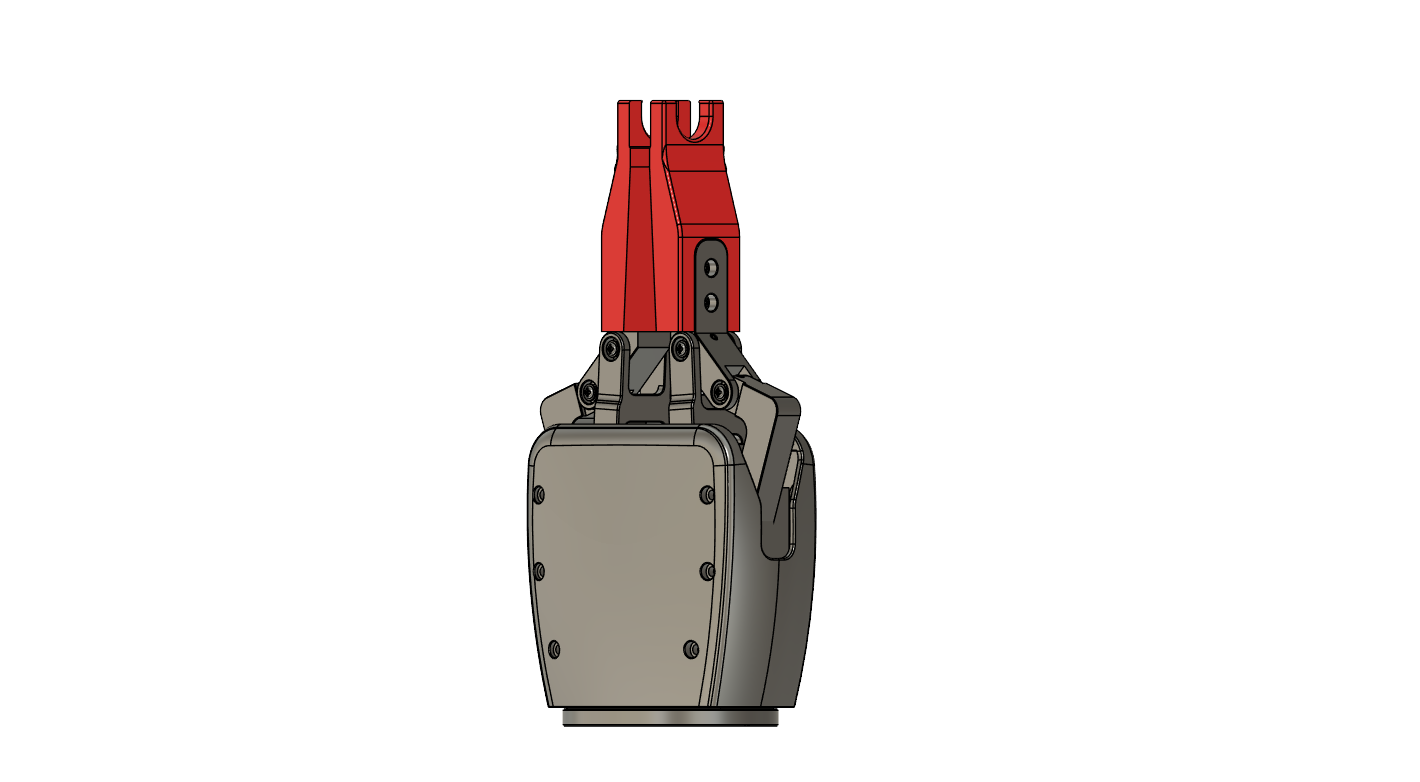
\includegraphics[width=0.8\textwidth]{assets/figures/Pince_Xarm6.png}
    \caption{Pince du bras robot Ufactory Xarm6 modifiée pour la prise de pièces}
    \label{fig:pince_robot}
\end{figure}

En rouge, les doigts offrent une visibilité optimale pour la caméra et permettent une prise plus précise qu'avec des doigts sans modification. Imprimées en 3D, ces pièces sont suffisamment robustes pour prendre les pièces sans les lâcher mais sont suffisamment fragiles pour céder en cas de contact fortuit avec des autres éléments de la maquette.

\section{Graveuse laser Creality Falcon}

La graveuse laser Creality Falcon a été choisie comme graveuse laser car elle offre une bonne qualité de gravure, une bonne vitesse et une puissance correcte par rapport à son prix. De plus, cette graveuse est compatible avec des fichiers G-code, et il est également possible d'envoyer les instructions ligne par ligne via la connexion USB-C, ce qui permet un contrôle plus fin et interactif du processus de gravure. Cette fonctionnalité sera utilisée plus tard pour le contrôle de la graveuse avec AICA Studio

\subsection{Utilisation}
La graveuse laser Creality Falcon est commandée via des fichiers G-code, un langage standard dans le domaine des machines-outils à commande numérique. Les motifs à graver, initialement créés au format \gls{dxf}, sont convertis en fichiers G-code via un script développé spécialement dans le cadre de ce projet.

Ce script réalise les étapes suivantes :
\begin{itemize}
    \item Lecture et analyse des contours du fichier DXF.
    \item Génération de trajectoires compatibles avec le protocole G-code.
    \item Communication entre le logiciel et la graveuse laser.
\end{itemize}

Le fichier G-code généré est ensuite envoyé à la Creality Falcon qui réalise la gravure. Une synchronisation précise avec le bras robot est nécessaire pour assurer que le laser ne s'active que lorsque le bras est en position correcte.

\subsection{Modifications}

Afin que la graveuse laser s'intègre bien dans la maquette et que le robot puisse se positionner correctement sous la tête laser, des pieds personnalisés ont été conçus en 3D afin de réhauser la graveuse. Ces pieds permettent également de fixer l'ensemble de la machine à la table afin de minimiser les problèmes de précision.

\section{Écran tactile ED-HMI3010-101C}

L’écran tactile ED-HMI3010-101C (appelé ED-101) permet de choisir ce que la graveuse va dessiner. Via une interface graphique, il est possible de dessiner à la main, avec des formes prédéfinies ou avec du texte dans la zone de gravure.
Cet écran a été choisi car il repose sur une raspberry Pi 5 pour fonctionner. Cela offre une facilité d'intégration car la documentation de l'écran et de la carte éléctronique est très fournie et très complète. De plus, l'utilisation de l'ensemble est relativement simple du fait que l'écran tactile ne nécessite pas de souris ou de clavier.

La création de l'interface graphique a été programmée sur un ordinateur annexe et ensuite transféré sur la Raspberry Pi 5 pour faciliter le débogage et le téléchargement inutile de logiciels sur la carte éléctronique.

Cette interface est spécialement conçue pour une utilisation en tant que démonstrateur devant du public.

\section{Caméra Intel D435}

La caméra Intel D435 est utilisée pour la détection en 3D des pièces à graver dans l’espace de travail. Grâce à sa capacité à fournir des données de profondeur en temps réel, elle permet :
\begin{itemize}
    \item De localiser précisément les pièces posées sur la zone de travail.
    \item D’adapter la trajectoire du bras robot en fonction de la position exacte des pièces détectées.
\end{itemize}

L’intégration de la caméra dans le système est réalisée via un bloc fonctionnel personnalisé développé dans AICA Studio, utilisant les données 3D captées pour prendre des décisions en temps réel. Le fonctionnement détaillé de ce bloc sera présenté dans le \textbf{chapitre \ref{chap:programmation}}.

\subsection{Positionnement de la caméra}

Tout comme les doigts du robot et les pieds de la graveuse laser, la caméra à bénéficié d'un support d'accrochage imprimé en 3D. Ce support permet un positionnement précis et robuste ainsi qu'un rendu ésthétique agréable dans le même style que les pieds de la graveuse.

\begin{figure}[H]
    \centering
    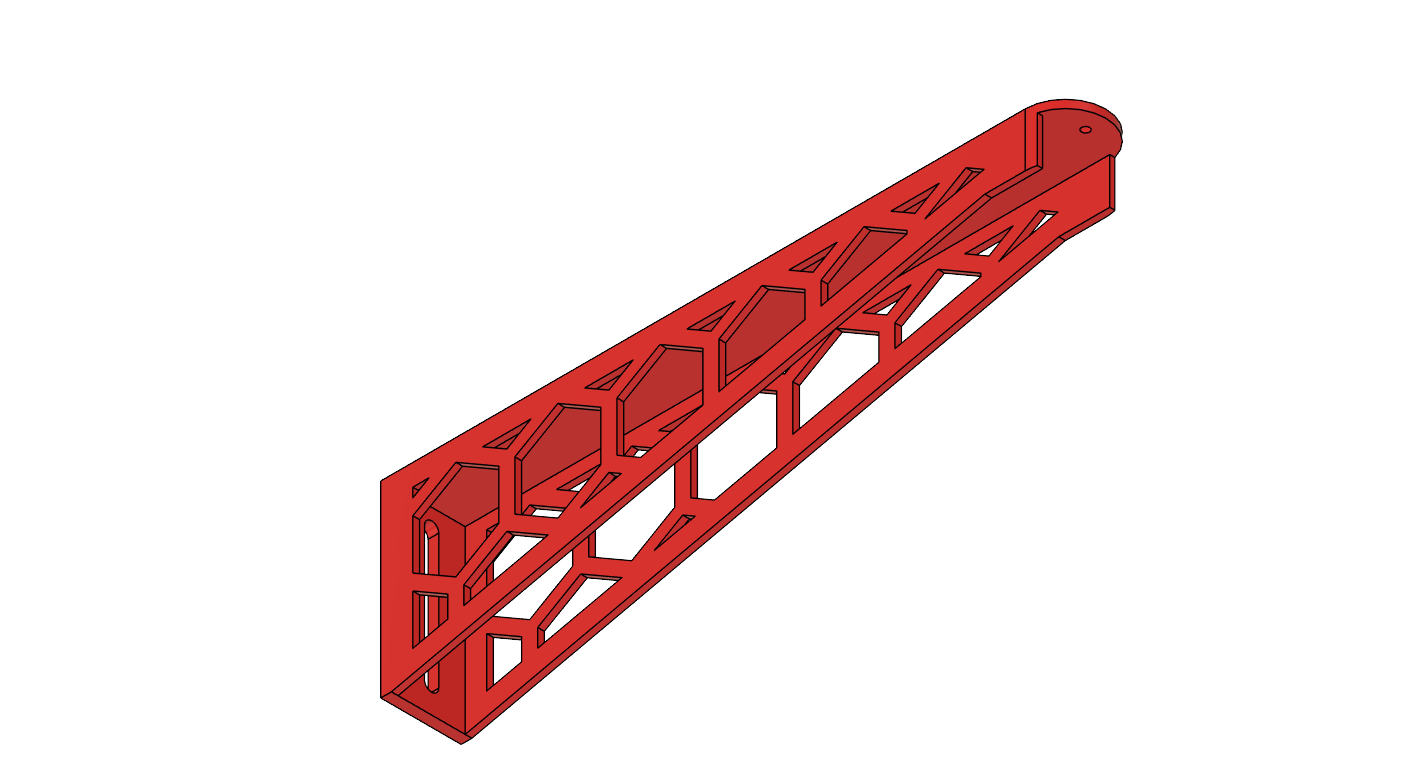
\includegraphics[width=0.8\textwidth]{assets/figures/Porte_camera v6.png}
    \caption{Support d'accrochage de la caméra Intel D435}
    \label{fig:support_camera}
\end{figure}

Ce support permet aussi de faire passer le cable d'alimentation et de communication proprement le long de la structure de la maquette.


\section{Modèle 3D de la maquette}

Le modèle 3D de la maquette a été réalisé à l'aide du logiciel de modélisation 3D Fusion 360. Il permet de visualiser l'ensemble du système, y compris le bras robot, la graveuse laser, l'écran tactile et la caméra. Ce modèle est utilisé dans AICA Studio pour la visualisation de l'espace de travail et le placement des points de passage du robot.

\begin{figure}[H]
    \centering
    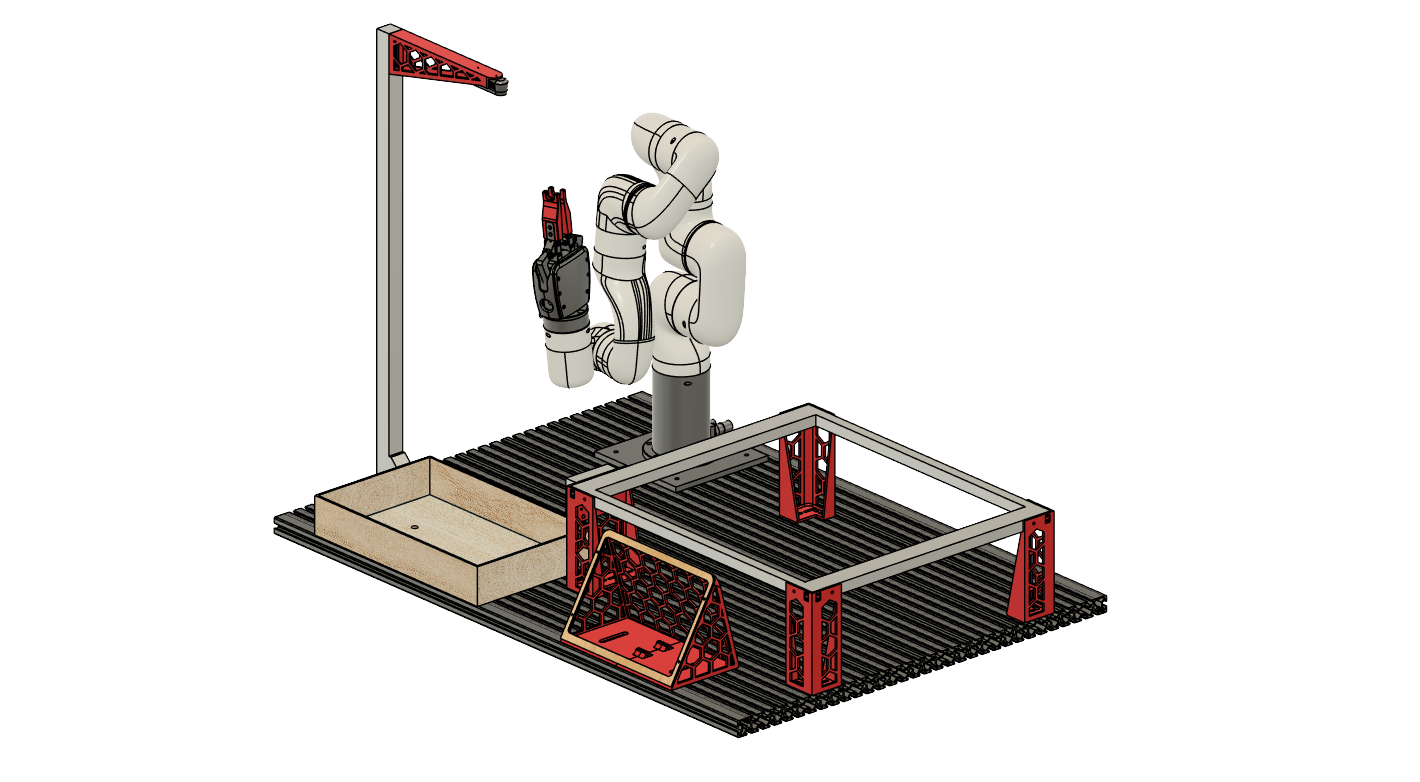
\includegraphics[width=0.8\textwidth]{assets/figures/modele_3d.png}
    \caption{Modèle 3D de la maquette de la graveuse laser intelligente}
    \label{fig:maquette_3d}
\end{figure}

Ce travail de modélisation a été réalisé pour faciliter la conception de pièces mécaniques, et la définition des points de passage du bras robot. Cela évite des erreurs de mesures et permet de mieux visualiser l'ensemble du système avant la fabrication des pièces ainsi que l'encombrement de la maquette.

En plus de cela, cette maquette à permis de calculer avec précision la transformation entre le repère caméra et le repère monde utilisé dans le programme de reconaissance de pièce. Cette partie sera détaille dans le \textbf{chapitre \ref{chap:programmation}}.
